% !TEX root = ./TransportFR.tex


\newcommand{\Blu}[1]{{\color{blue}#1}}
\newcommand{\Red}[1]{{\color{red}#1}}
\newcommand{\iC}{\Red{i}}
\newcommand{\jC}{\Blu{j}}
\newcommand{\aC}{\Red{a}}
\newcommand{\bC}{\Blu{b}}


\ifdefined\otarticle
\newcommand{\myparagraph}[1]{\subsection{#1}}
\else
\newcommand{\myparagraph}[1]{\paragraph{#1}}
\chapter{Le Transport Optimal et ses Applications}
\fi

\label{chap-ot}


%%%%%%%%%%%%%%%%%%%%%%%%%%%%%%%%%%%%%%%%%%%%%%
\section{Le Transport Optimal de Monge}

Gaspard Monge, en plus d'être un grand mathématicien, a participé activement à la révolution Française, et a créé l'\'Ecole Polytechnique ainsi que l'\'Ecole Normale Supérieure. Motivé par des applications militaires, il a formulé en 1781 le problème du transport optimal~\cite{Monge1781}. Il s'est posé la question du calcul de la façon la plus économique de transporter de la terre entre deux endroits pour faire des remblais. Dans son texte original, il a fait l'hypothèse que le coût du déplacement d'une unité de masse est égal à la distance parcourue, mais on peut utiliser n'importe quel coût adapté au problème à résoudre. 

%%%%%%%%%%%%%%%%%%%%%%%%%%%%%%%%%%%%%%%%%%%%%%%%%%%%%
\myparagraph{Le problème de Monge}

Pour illustrer le problème et sa formulation mathématique, intéressons-nous à la façon optimale de distribuer les croissants depuis les boulangeries vers les cafés, le matin dans Paris. Pour simplifier, nous allons supposer qu'il y a uniquement six boulangeries et cafés, que l'on peut voir à la figure~\ref{fig:image-cafe} (les boulangeries sont en \Red{rouge} et les cafés en \Blu{bleu}). Le coût à minimiser est le temps total des trajets, et l'on note $C_{\iC,\jC}$ le temps entre la boulangerie $\iC \in \{1,\ldots,6\}$  et le café $\jC \in \{1,\ldots,6\}$. Par exemple, on a $C_{\Red{3},\Blu{4}}=10$, ce qui signifie qu'il y a dix minutes de trajet entre la boulangerie numéro $\Red{3}$ et le café numéro $\Blu{4}$. 

\begin{figure}\centering
    \begin{tabular}{@{}c@{\hspace{1mm}}c@{\hspace{4mm}}c@{\hspace{1mm}}c@{}}
        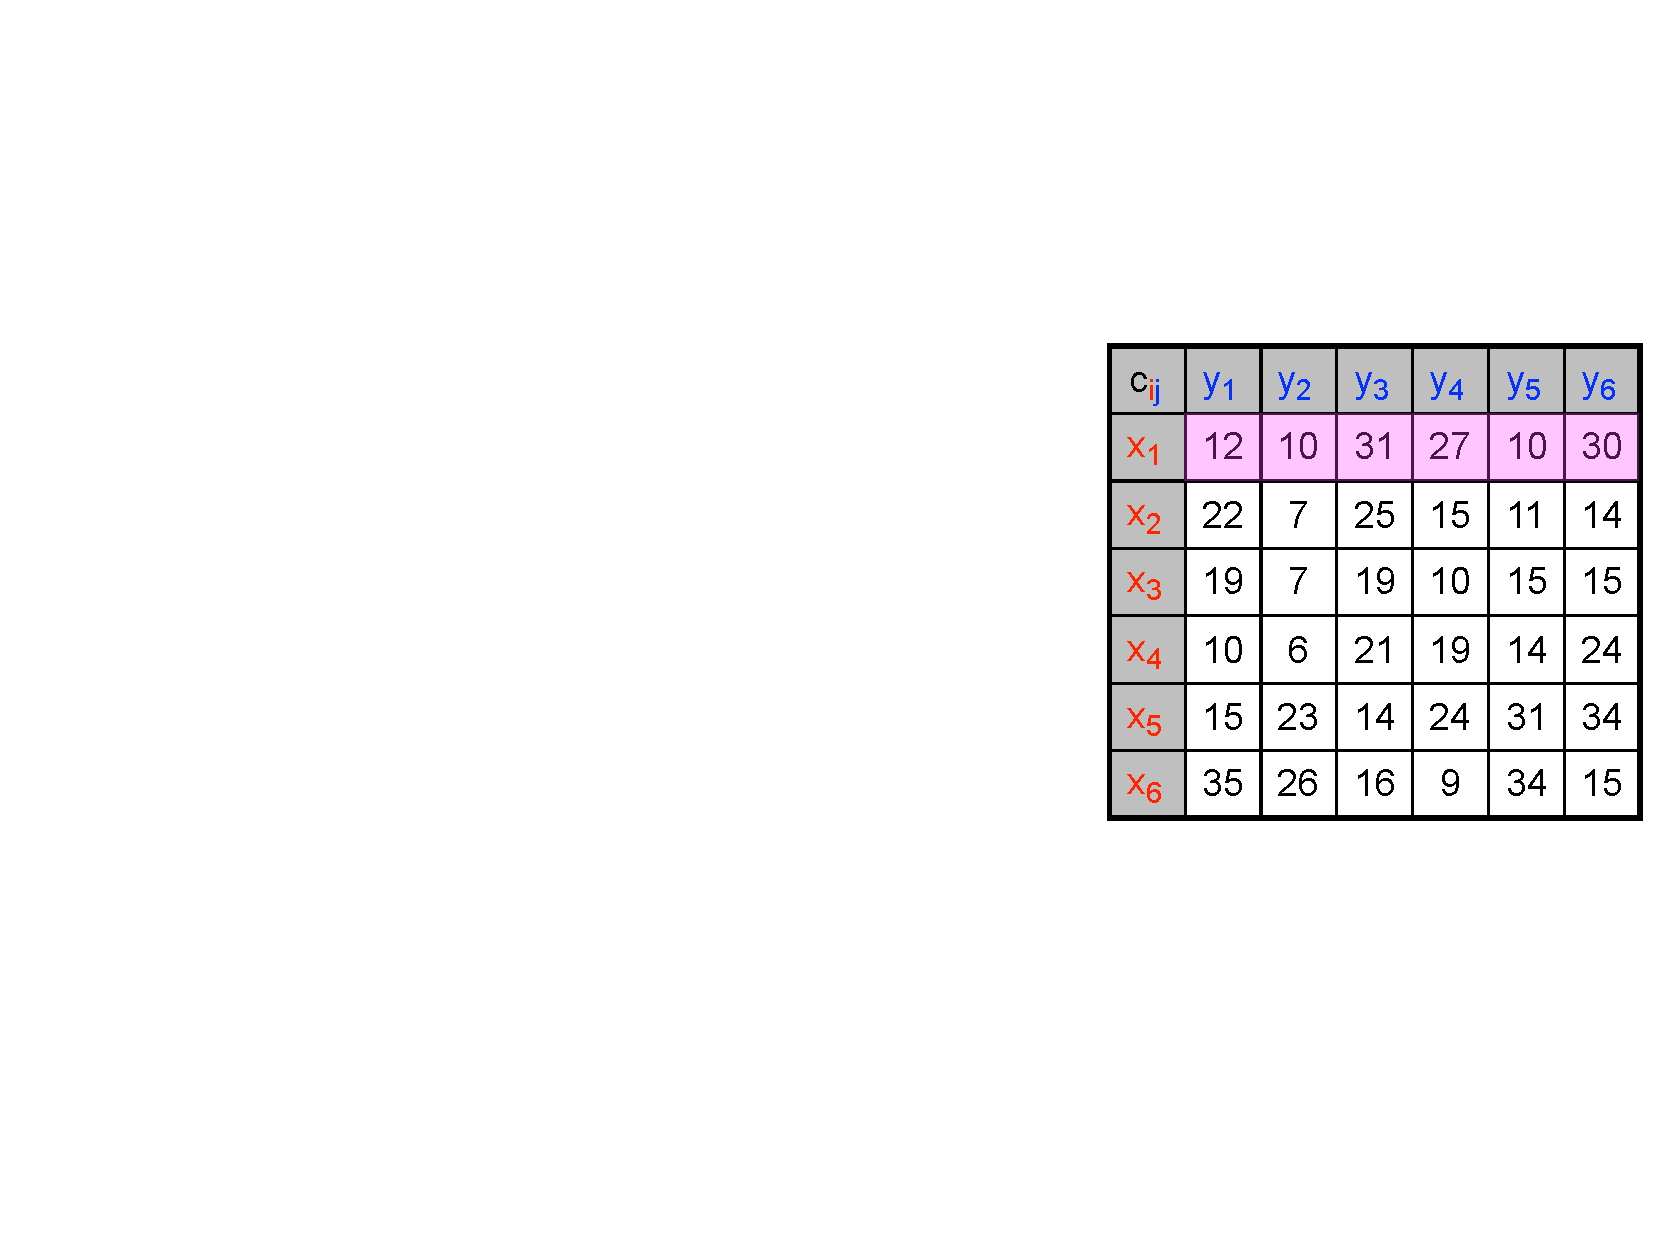
\includegraphics[width=.22\linewidth]{transport/cafe-paris/map-paris-0-couts} 
        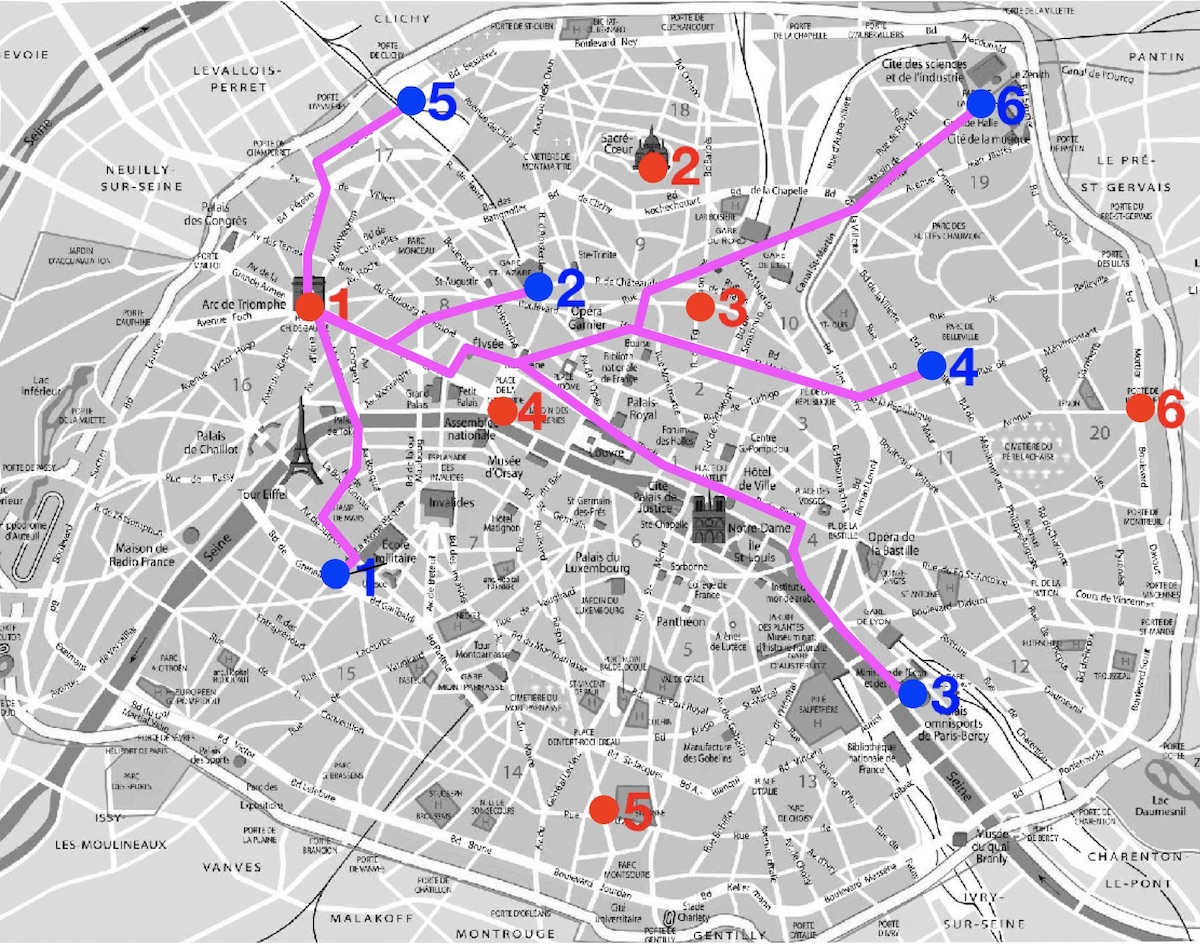
\includegraphics[width=.27\linewidth]{transport/cafe-paris/map-paris-0} 
        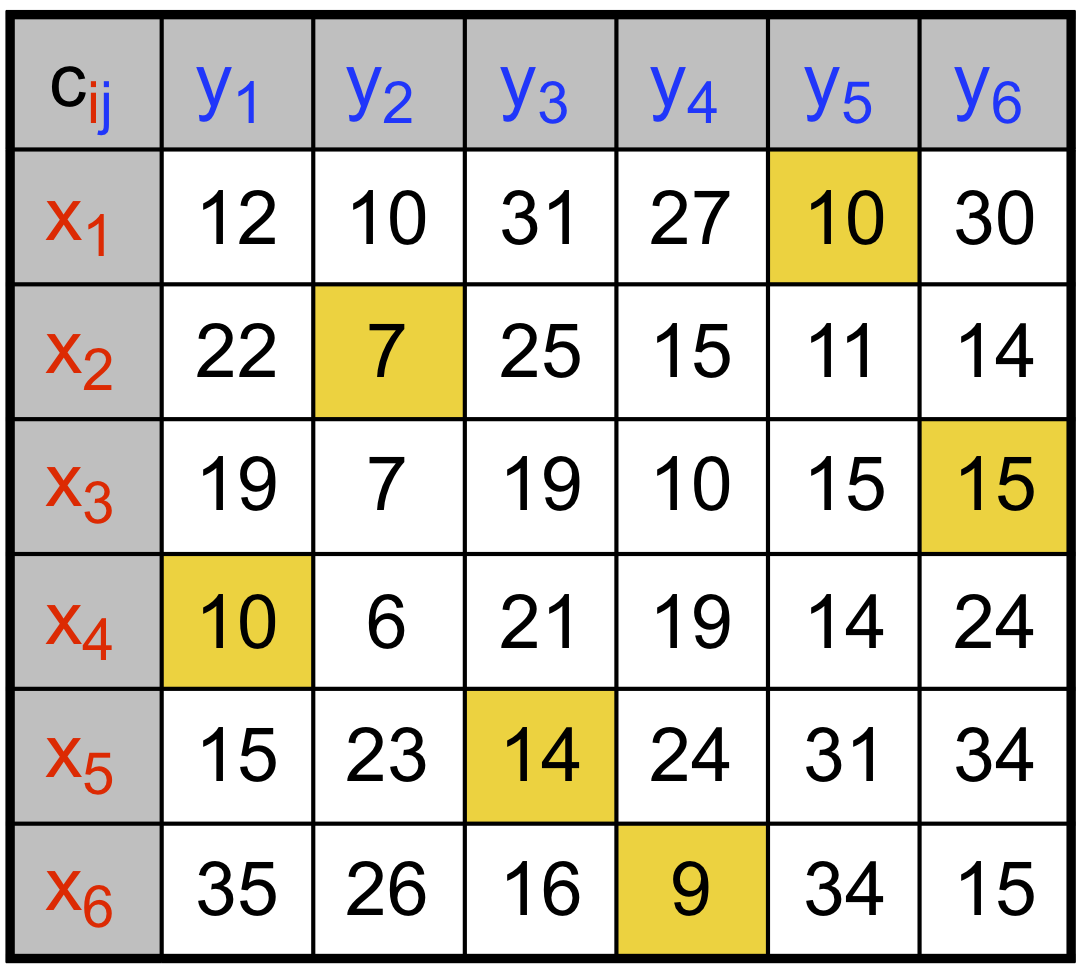
\includegraphics[width=.22\linewidth]{transport/cafe-paris/map-paris-1-couts} 
        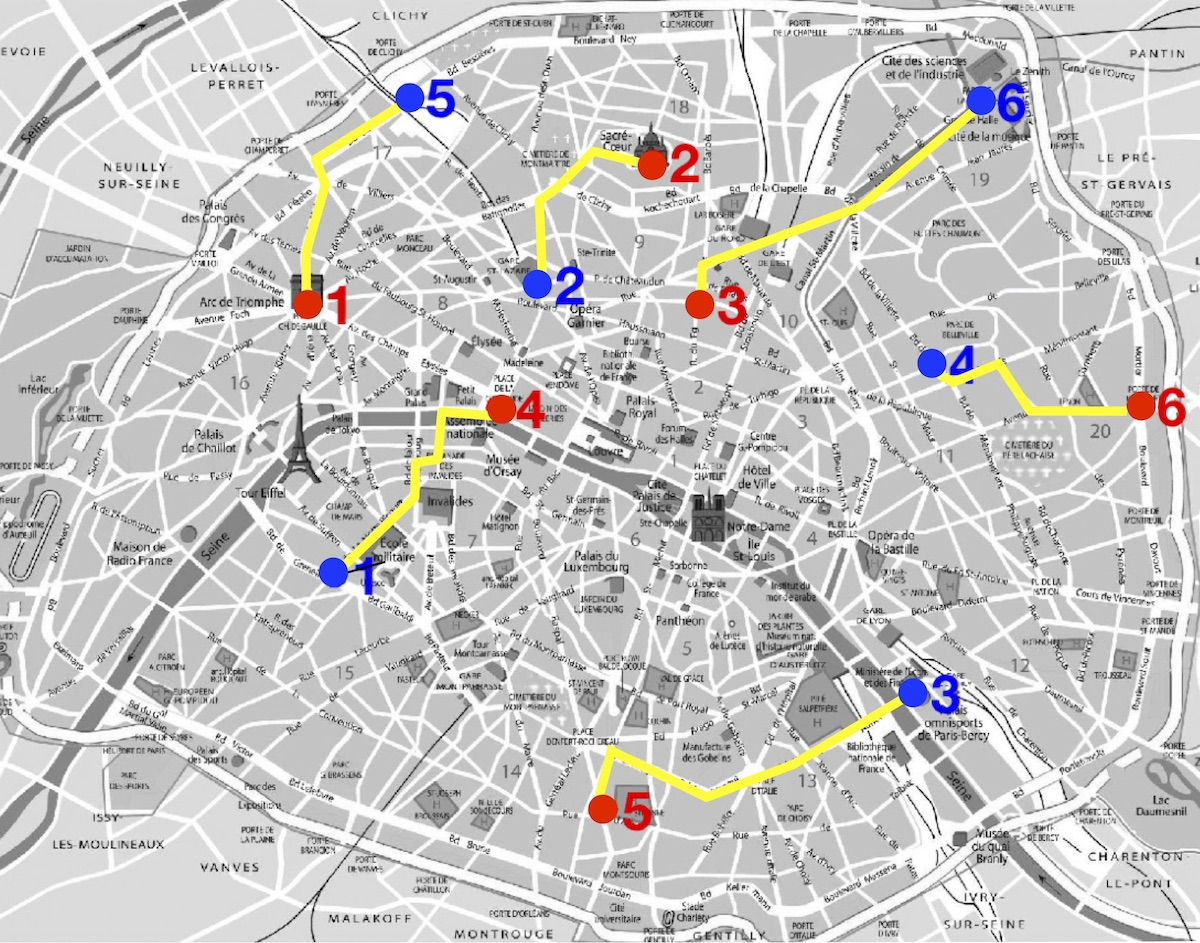
\includegraphics[width=.27\linewidth]{transport/cafe-paris/map-paris-1} 
    \end{tabular}
    \caption{\label{fig:image-cafe} Matrice de coût et connexions associées. Gauche : une ligne de la matrice coût. Droite : un exemple particulier de permutation. } 
\end{figure}

Afin de satisfaire la contrainte d'approvisionnement (que l'on appelle aussi la conservation de la masse), il faut que chaque boulangerie soit connectée à un et un seul café. Comme il y a le même nombre de boulangeries que de cafés, ceci implique que chaque café est également connecté à une et une seule boulangerie. On va noter 
\eq{    
    \si : \iC \in \{1,\ldots,6\} \longmapsto \jC \in \{1,\ldots,6\}
}
un tel choix de connexions. La figure~\ref{fig:image-cafe} illustre au centre et à droite l'exemple
\eql{\label{eq-bijection-exmp}
    \si(\Red{1})=\Blu{5}, \;
    \si(\Red{2})=\Blu{2}, \;
    \si(\Red{3})=\Blu{6}, \;
    \si(\Red{4})=\Blu{1}, \;
    \si(\Red{5})=\Blu{3}, \;
    \si(\Red{6})=\Blu{4}.
}  
La contrainte de conservation de masse signifie que $\si$ est une bijection de l'ensemble $\{1,\ldots,6\}$ dans lui-même. On dit aussi que $\si$ est une permutation. 

Le coût de transport associé à une telle bijection est la somme des coûts $C_{\iC,\si(\iC)}$ sélectionnés par la permutation $\si$, c'est-à-dire 
\eql{\label{eq:cout}
    \text{Coût}(\si) \eqdef 
        C_{\Red{1},\si(\Red{1})} + 
        C_{\Red{2},\si(\Red{2})} + 
        C_{\Red{3},\si(\Red{3})} + 
        C_{\Red{4},\si(\Red{4})} + 
        C_{\Red{5},\si(\Red{5})} + 
        C_{\Red{6},\si(\Red{6})}. 
}
Par exemple, pour la bijection~\eqref{eq-bijection-exmp} montrée à la figure~\ref{fig:image-cafe}, on obtient comme coût
\eq{
    C_{\Red{1},\Blu{5}} + 
    C_{\Red{2},\Blu{2}} + 
    C_{\Red{3},\Blu{6}} + 
    C_{\Red{4},\Blu{1}} + 
    C_{\Red{5},\Blu{3}} + 
    C_{\Red{6},\Blu{4}} = 
    10 + 7 + 15 + 10 + 14 + 9 = 65. 
}


Le problème de Monge consiste à chercher la permutation $\si$ qui a le coût minimum, c'est-à-dire résoudre le problème d'optimisation
\eql{\label{eq:monge}
    \umin{\si \in \Si_6} \text{Coût}(\si), 
}
où 
l'on a noté $\Si_6$ 
l'ensemble des permutations de l'ensemble $\{1,\ldots,6\}$.

\begin{figure}\centering
    \begin{tabular}{@{}c@{\hspace{1mm}}c@{\hspace{1mm}}c@{\hspace{1mm}}c@{}}
        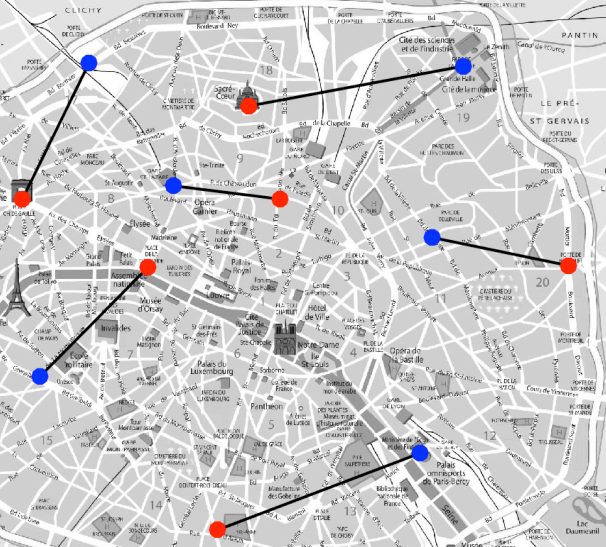
\includegraphics[width=.22\linewidth]{transport/cafe-paris/ordre-croissant-64}&
        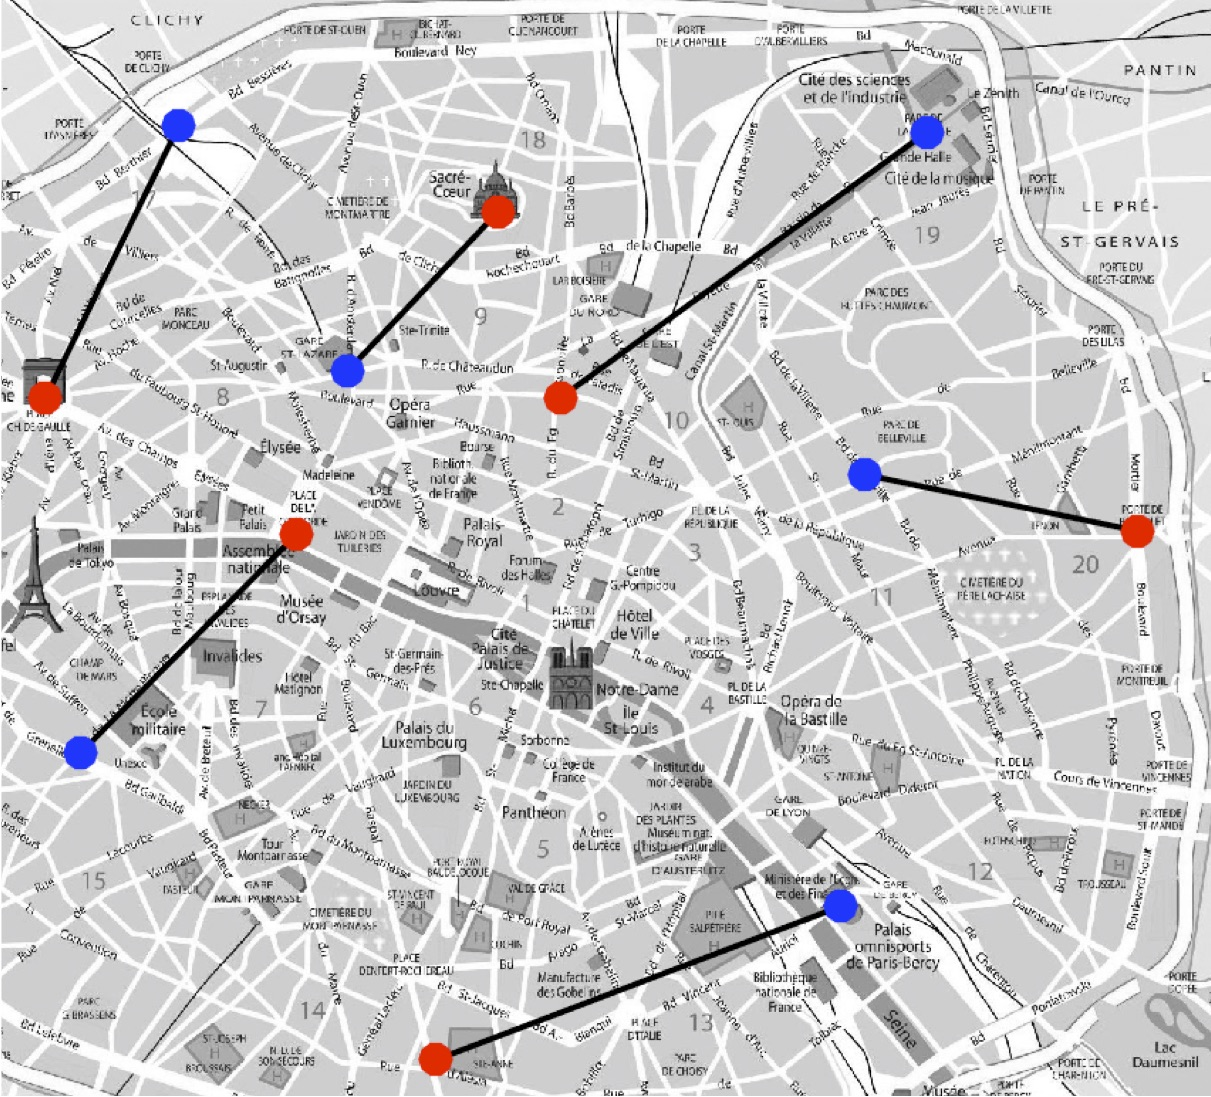
\includegraphics[width=.22\linewidth]{transport/cafe-paris/ordre-croissant-65}&
        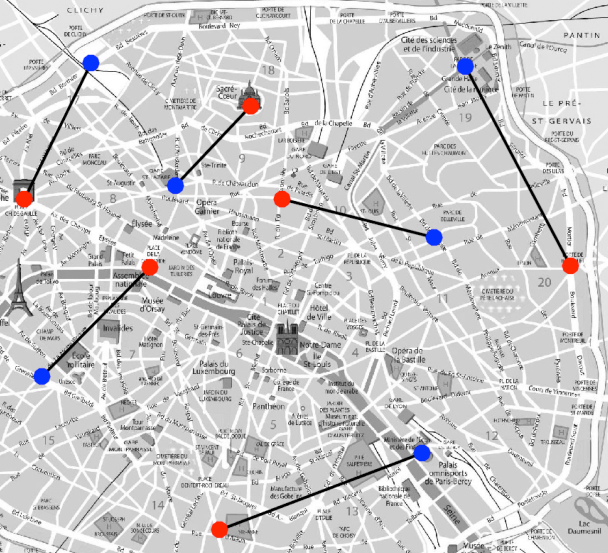
\includegraphics[width=.22\linewidth]{transport/cafe-paris/ordre-croissant-66}&
        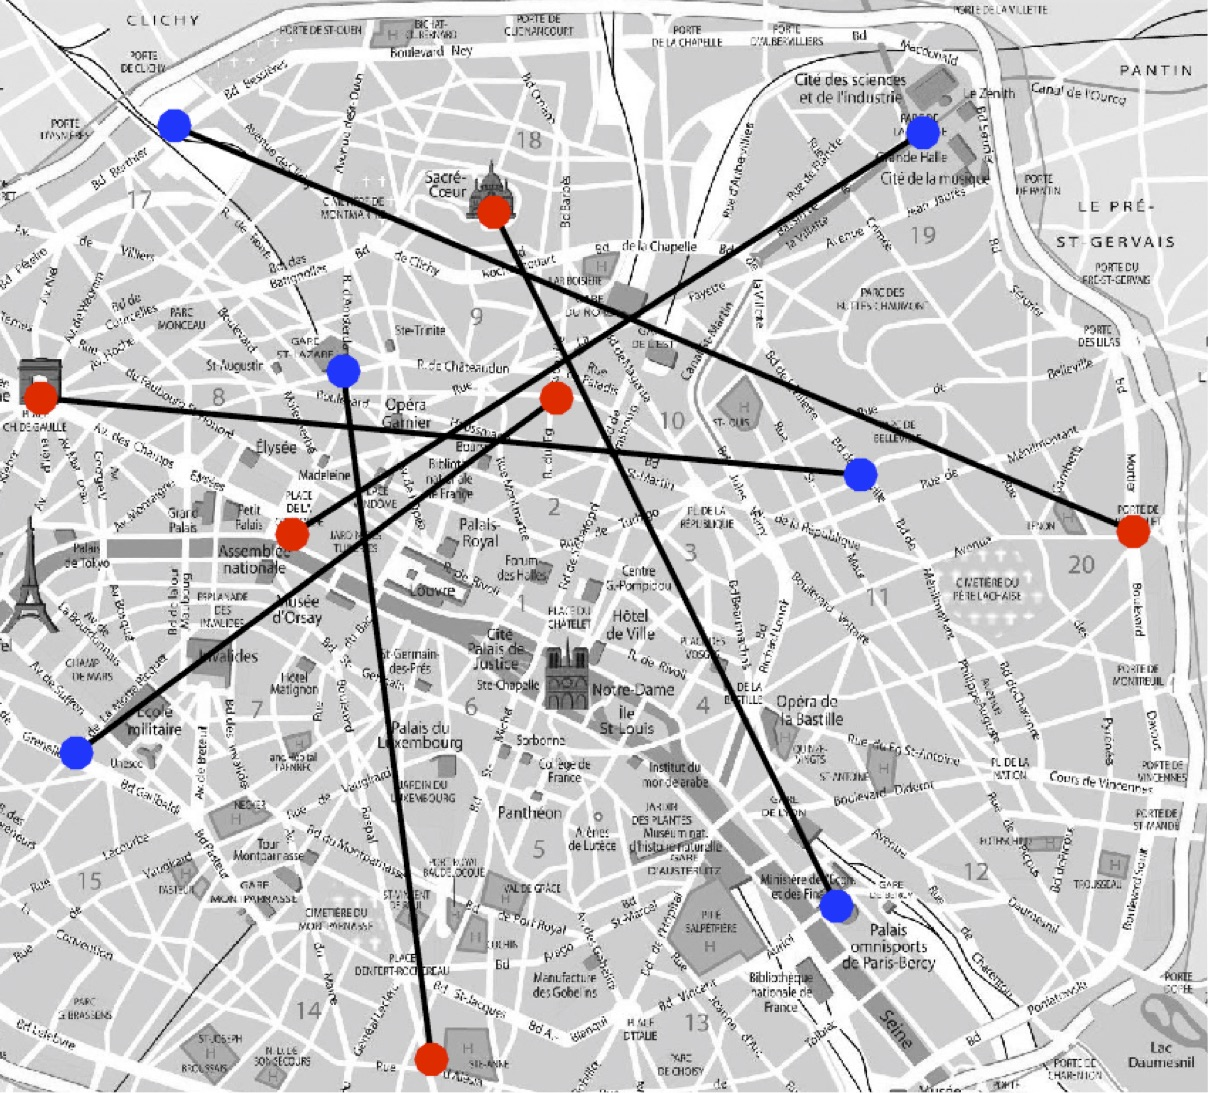
\includegraphics[width=.22\linewidth]{transport/cafe-paris/ordre-croissant-152}\\
        Coût=64 &  
        Coût=65 &  
        Coût=66 &  
        Coût=152
    \end{tabular}
    \caption{\label{fig:ordre-croissant} Exemples de permutations avec différent coûts. } 
\end{figure}

La figure~\ref{fig:ordre-croissant} montre que la permutation~\eqref{eq-bijection-exmp} n'est pas la meilleure : il existe par exemple une autre permutation qui a un coût de 64. Mais est-ce la meilleure ? Il se trouve que oui, on peut en effet tester sur un ordinateur toutes les permutations de  $\{1,\ldots,6\}$ et calculer leur coût. Combien y a-t-il de permutations au total ? Pour effectuer ce dénombrement, on voit qu'il y a six choix d'affectation possible de $\Red{1}$ à  $\si(\Red{1}) \in \{\Blu{1,\ldots,6}\} $, puis cinq choix possibles pour affecter $\Red{2}$ à $\si(\Red{2}) \in  \{ \Blu{1,\ldots,6 } \}  - \{ \si(\Red{1}) \}$, et ainsi de suite. Le nombre total de possibilités est donc $6 \times 5 \times 4 \times 3 \times 2 \times 1 = 720$ que l'on note $6!$, \guill{factorielle 6}. Si on considère un nombre $n$ de boulangeries, alors le nombre de permutations à tester pour trouver la meilleure est $n! =n \times (n-1) \times \ldots \times 2 \times 1$. Ce nombre croit extrêmement vite avec $n$, par exemple $70! \approx 1,198 \times 10^{100}$, à comparer avec les $10^{11}$ neurones dans le cerveau et les $10^{79}$ atomes dans l'univers. Cette stratégie de recherche exhaustive n'est donc possible que pour de toute petites valeurs de $n$. 


\begin{figure}\centering
    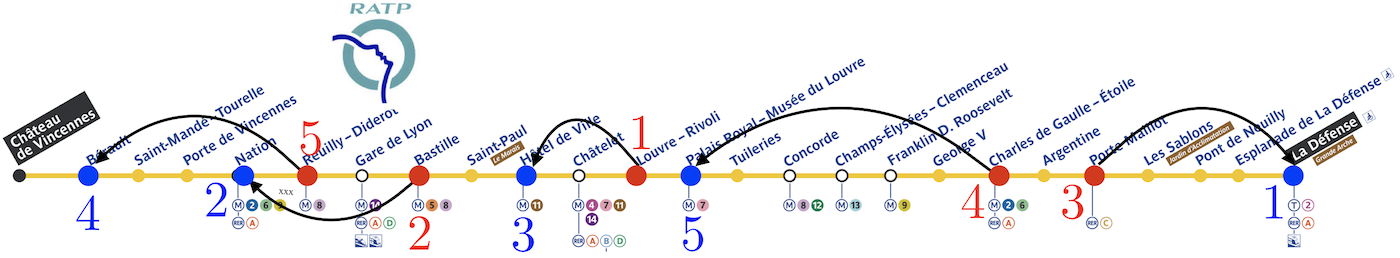
\includegraphics[width=.7\linewidth]{transport/metro/plan-metro}
    \caption{\label{fig:metro} Le transport optimal en 1D le long d'une ligne de métro. La bijection optimale est  
    $\si : (\Red{1,2,3,4,5}) \mapsto (\Blu{3,2,1,5,4})$. } 
\end{figure}

%%%%%%%%%%%%%%%%%%%%%%%%%%%%%%%
\myparagraph{En 1D et 2D}

La section~\ref{sec-kanto} explique comment des avancées mathématiques ont permis de développer des techniques efficaces pour calculer un transport optimal $\si$ même pour de grandes valeurs de $n$. Mais il aura fallu attendre près de 200 ans pour y arriver. Dans certains cas simples, on peut cependant calculer le transport optimal de façon simple. Le cas le plus élémentaire est lorsque les points à apparier sont le long d'un axe 1D, par exemple si les cafés et les boulangeries sont situés le long d'une ligne de métro. Il faut également que le coût $C_{\iC,\jC}$ soit la distance le long de cet axe (par exemple le temps de trajet en métro entre les stations). Dans ce cas, il suffit de classer les indices $\iC$ et $\jC$ par ordre croissant (donc de gauche à droite le long de la ligne de métro) et d'apparier le premier indice $\iC$ au premier indice $\jC$ ensemble, puis le deuxième indice, etc. Ce procédé est illustré à la figure~\ref{fig:metro}.  Le temps de calcul nécessaire pour calculer le transport optimal en métro est donc le temps nécessaire pour classer les indices. L'algorithme le plus simple pour effectuer un classement est celui utilisé habituellement pour trier un jeu de $n$ cartes : il s'agit du tri par insertion, qui insère itérativement chaque carte à sa place par rapport aux cartes déjà classées. Il effectue $n(n-1)/2$ comparaisons. Pour $n=70$, ceci nécessite donc seulement 21415 operations, ce qui rend la méthode utilisable, au contraire de la recherche exhaustive de toutes les $n!$ permutations.
% 
On dispose d'algorithmes encore plus rapides (par exemple le tri fusion), qui effectuent de l'ordre de $n \log(n)$ opérations, et donc pour $n = 70$, de telles méthodes nécessitent moins de 1000 opérations. 

Malheureusement, il n'est plus possible d'utiliser cette technique de classement dans des cas plus généraux. Pour des points en dimension 2, si on prend comme coût $C_{\iC,\si(\iC)}$ la distance euclidienne (la distance en vol d'oiseau) entre les points, alors Gaspard Monge a montré dans son papier original (voir la figure~\ref{fig:ot2d}, à gauche) qu'un transport optimal ne peut par contenir de croisement. Par exemple, comme le montre la figure~\ref{fig:ot2d} (à droite), si l'on trace tous les segments entre les points $\iC \mapsto \jC = \si(\iC)$  que l'on relie par la bijection définie par un $\si$ optimal, ceux-ci ne se croisent jamais. 

\begin{figure}\centering
    \begin{tabular}{@{}c@{\hspace{6mm}}c@{\hspace{3mm}}c@{}} % c@{\hspace{1mm}}
        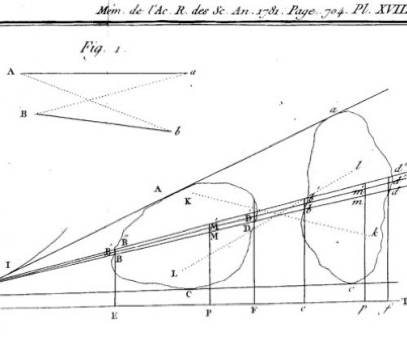
\includegraphics[width=.22\linewidth]{transport/monge-2d/article-monge}&
%        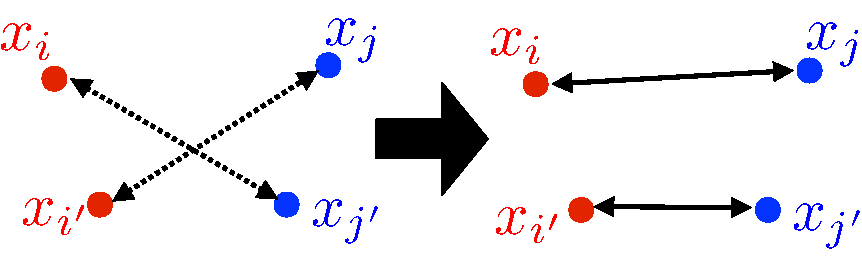
\includegraphics[width=.22\linewidth]{transport/monge-2d/decroisement}&
        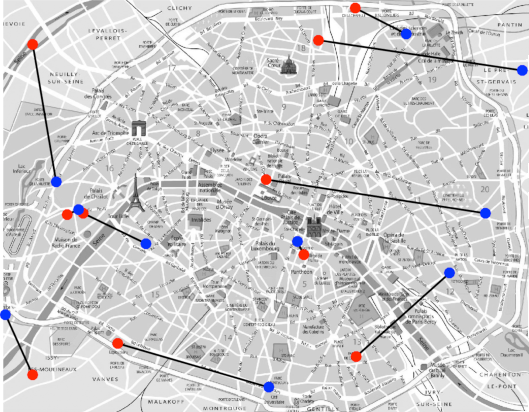
\includegraphics[width=.22\linewidth]{transport/monge-2d/example-10}&
        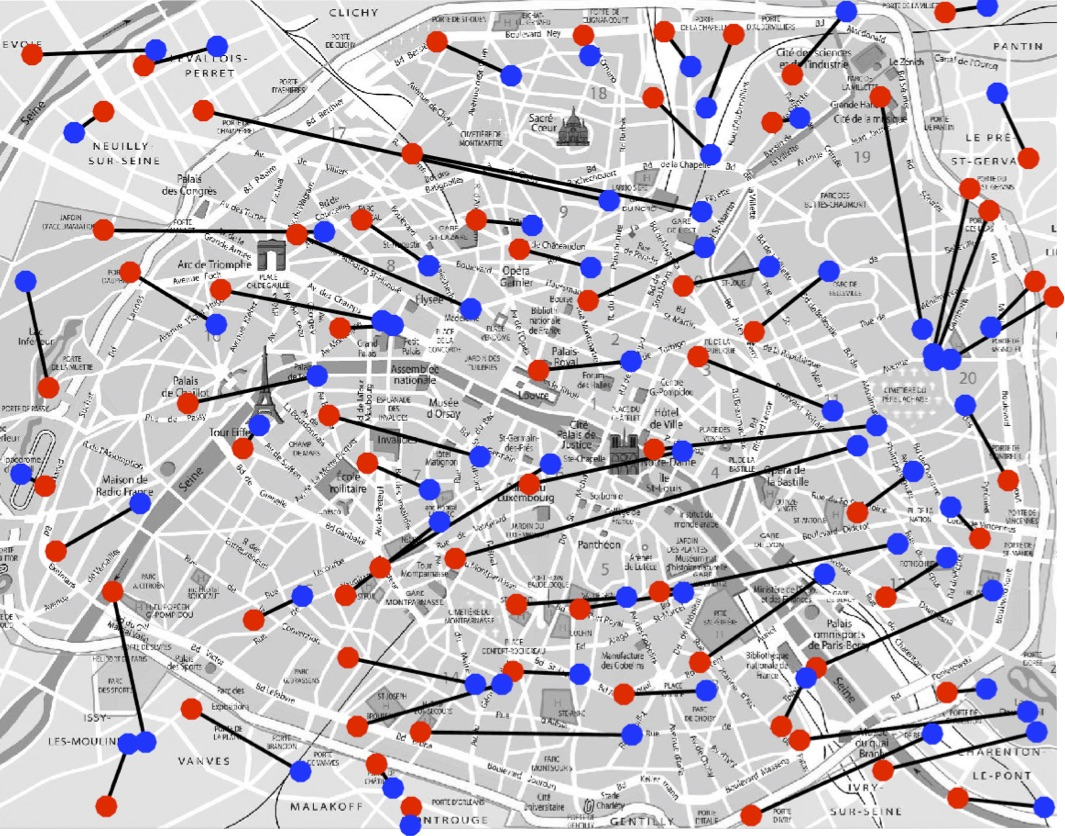
\includegraphics[width=.22\linewidth]{transport/monge-2d/example-70}
    \end{tabular}
    \caption{\label{fig:ot2d} Gauche: extrait de l'article de Monge~\cite{Monge1781}. Droite: le transport optimal en 2D pour un coût euclidien.  } 
\end{figure}

Cette observation géométrique n'est cependant pas suffisante pour calculer un transport optimal en 2D : il existe en effet beaucoup de permutations $\si$ telles que les segments associés ne se croisent pas. 
%
Il va falloir analyser de façon plus fine la structure des permutations optimales afin de pouvoir les calculer de façon efficace. 
%
Nous allons maintenant voir comment Leonid Kantorovitch a reformulé le problème de Monge afin d'y parvenir. 


%%%%%%%%%%%%%%%%%%%%%%%%%%%%%%%%%%%%%%%%%%%%%%
\section{Le Transport Optimal de Kantorovitch}
\label{sec-kanto}

Leonid Kantorovitch est un mathématicien et un économiste soviétique qui a révolutionné la théorie du transport optimal pendant les années 40. Ses recherches sont issues de considérations pratiques qui l'ont occupé avant et après la seconde guerre mondiale. Il y a joué un rôle important pour assurer une distribution optimale des ressources, en particulier durant le siège de Léningrad.
%
Il a par la même occasion participé au développement de l'optimisation moderne, laquelle a eu un impact énorme dans de très nombreux domaines appliqués. Il a ainsi obtenu en 1975 le prix Nobel d'économie, car les premières applications (mais certainement pas les seules !) de sa théorie l'ont été dans ce domaine. 


%%%%%%%%%%%%%%%%%%%%%%%%%%%%%%%
\myparagraph{Le problème de Kantorovitch}

L'idée centrale de Kantorovitch est de modifier le problème de Monge en remplaçant l'ensemble des permutations par un ensemble plus grand mais plus simple. Tout d'abord on remarque que l'on peut représenter une permutation $\si \in \Si_n$ à l'aide d'une matrice de permutation $P$ qui est une matrice binaire (remplie de 0 et de 1) de taille $n \times n$ telle que $P_{\iC,\jC} = 0$ sauf si $\jC=\si(\iC)$ auquel cas $P_{\iC,\si(\iC)} = 1$. Par exemple, pour $n=3$ points, les permutations 
$(\Red{1,2,3}) \mapsto (\Blu{1,2,3})$ (l'identité), 
$(\Red{1,2,3}) \mapsto (\Blu{3,2,1})$ et
$(\Red{1,2,3}) \mapsto (\Blu{2,1,3})$ sont représentées par les matrices de taille $3 \times 3$
\eq{
	\begin{pmatrix} 1&0&0 \\ 0&1&0 \\ 0&0&1 \end{pmatrix}, \quad
	\begin{pmatrix} 0&0&1 \\ 0&1&0 \\ 1&0&0 \end{pmatrix} \qetq
	\begin{pmatrix} 0&1&0 \\ 1&0&0 \\ 0&0&1 \end{pmatrix}.
}
Dans la suite, on note $\Pp_n$ l'ensemble des $n!$ matrices de permutation de taille $n \times n$.

Comme la matrice est binaire, avec seulement $n$ éléments non-nuls égaux à 1, on peut remplacer la somme de $n$ termes qui apparait dans $\text{Coût}(\si)$ défini en~\eqref{eq:cout} par une somme sur l'ensemble des $n \times n$ indices $(\iC,\jC)$, c'est-à-dire que si $P$ est la matrice de permutation associée à $\si$, on a 
\eq{
	\text{Coût}(\si) = \sum_{\iC=1}^n \sum_{\jC=1}^n P_{\iC,\jC} C_{\iC,\jC}.
}
On peut ainsi remplacer le problème de Monge~\eqref{eq:monge} par le problème équivalent 
\eql{\label{eq:mongematrix}
    \umin{P \in \Pp_n}  \sum_{\iC=1}^n \sum_{\jC=1}^n P_{\iC,\jC} C_{\iC,\jC}.
}

Le génie de Kantorovitch a été de remarquer que l'on peut remplacer l'ensemble discret $\Pp_n$ (c'est-à-dire composé d'un ensemble fini, mais très grand, de $n!$ matrices) par un ensemble \guill{continu} (donc en particulier infini) mais plus simple. On remarque en effet que les matrices de permutation de $\Pp_n$ sont exactement les matrices qui ont un et un seul 1 le long de chaque ligne et de chaque colonne. Ceci peut aussi s'exprimer comme le fait qu'une matrice de permutation est une matrice binaire dont la somme de chaque ligne et de chaque colonne vaut 1, c'est-à-dire
\eq{
	\Pp_n = \enscond{ P \in \{0,1\}^{n \times n} }{ \foralls \iC, \sum_{\jC} P_{\iC,\jC}=1, \foralls \jC, \sum_{\iC} P_{\iC,\jC}=1  }.
}
Ce qui rend cet ensemble très compliqué, c'est la contrainte binaire, c'est-à-dire que ces matrices sont contraintes à être dans $\{0,1\}^{n \times n}$. Kantorovitch propose alors de \guill{relaxer} cette contrainte en supposant simplement que les entrées de $P$ sont entre $0$ et $1$. Ceci définit un ensemble plus grand, l'ensemble des matrices bistochastiques 
\eql{\label{eq:bistoch}
	\Bb_n \eqdef \enscond{ P \in [0,1]^{n \times n} }{ \foralls \iC, \sum_{\jC} P_{\iC,\jC}=1, \foralls \jC, \sum_{\iC} P_{\iC,\jC}=1  }.
}
Le problème de Kantorovitch s'obtient en effectuant ce remplacement dans~\eqref{eq:mongematrix}, afin de résoudre 
\eql{\label{eq:kantoassign}
    \umin{P \in \Bb_n} 
        \sum_{\iC=1}^n \sum_{\jC=1}^n P_{\iC,\jC} C_{\iC,\jC}.
}
L'immense avantage du problème de Kantorovitch~\eqref{eq:kantoassign} par rapport à celui de Monge~\eqref{eq:mongematrix} est que l'ensemble des matrices bistochastique est convexes, c'est-à-dire que si l'on considère deux matrices bistochastiques $P,Q \in \Bb_n$, alors leur moyenne $\frac{P+Q}{2} \in \Bb_n$ est encore bistochastique. Ceci n'est pas vrai pour les matrices de permutation, puisque la moyenne de deux matrices binaires $(P,Q)$ n'est pas binaire (sauf si bien sûr si $P=Q$). Cette convexité est la clef pour le développement d'algorithmes efficaces. 
%
Cette nouvelle formulation a en effet pu bénéficier d'une deuxième révolution initiée par George Dantzig~\cite{Dantzig51}, qui, à la même époque, a proposé l'algorithme du simplexe. Celui-ci permet de résoudre efficacement une certaine classe de problèmes d'optimisation convexe : les problèmes de programmation linéaire, dont~\eqref{eq:kantoassign} est un cas particulier. Dans le cas du problème de Kantorovitch, il existe en effet un algorithme du simplexe qui a une complexité de l'ordre de $n^3$ opérations, ce qui permet de faire des calculs pour de grands $n$, de l'ordre de plusieurs milliers. 


%%%%%%%%%%%%%%%%%%%%%%%%%%%%%%%
\myparagraph{L'équivalence Monge--Kantorovitch}

L'ensemble des matrices bistochastiques est plus grand que celui des matrices de permutations, $\Pp_n \subset \Bb_n$, de sorte que l'on a l'inégalité 
\eql{\label{eq:monge-vs-kanto}
    \umin{P \in \Bb_n} 
        \sum_{\iC=1}^n \sum_{\jC=1}^n P_{\iC,\jC} C_{\iC,\jC}
     \leq 
    \umin{P \in \Pp_n} 
        \sum_{\iC=1}^n \sum_{\jC=1}^n P_{\iC,\jC} C_{\iC,\jC}
}
entre les problèmes de Kantorovitch et de Monge. Mais de façon à première vue surprenante, un théorème fondamental dû à George Birkhoff et à John von Neumann~\cite{birkhoff,von1953certain} assure qu'en fait il y a égalité entre les valeurs de ces deux minimisations. En effet, ce théorème montre qu'il existe toujours une matrice solution du problème de Kantorovitch qui est une matrice de permutation, de sorte qu'elle est aussi solution du problème de Monge. Attention cependant, en général il n'y a pas unicité des solutions de ces problèmes : il peut exister une matrice bistochastique solution du problème de Kantorovitch qui n'est pas une permutation. 
%
La conjonction de deux avancées spectaculaires, dues à Kantorovitch et à Dantzig, a permis de rendre le transport optimal applicable à des problèmes de grande taille, puisque l'algorithme du simplexe permet de résoudre en pratique ces problèmes. 

%%%%%%%%%%%%%%%%%%%%%%%%%%%%%%%
\myparagraph{Le cas pondéré}

Outre son intérêt pratique, la formulation de Kantorovitch a aussi permis de généraliser le problème initial de Monge, en donnant le bon cadre pour le formaliser et l'étudier mathématiquement. En effet, le problème de Monge est très limité. Que se passe-t-il par exemple si il n'y pas le même nombre $n$ de cafés et $m$ de boulangeries ? Le problème initial~\eqref{eq:monge} n'a pas de solution, car on ne peut pas mettre en bijection deux ensembles de tailles différentes. Le bon concept n'est pas le nombre de boulangeries et de cafés, mais plutôt les distributions $(\Red{a_1,\ldots,a_n})$ de production (associées au boulangeries) et les distributions $(\Blu{b_1,\ldots,b_m})$ de consommation des cafés. 
%
Par exemple, si la première boulangerie produit 45 croissants par jour, on prendra $\Red{a_1} =45$, de même $\Blu{b_3} = 34$ signifie que le 3$^\text{e}$ café consomme 34 croissants par jour.
%
Dans le cas initialement considéré, où $n=m$, toutes les quantités $\Red{a_i}$ et $\Blu{b_j}$ sont égales à 1. Mais dans de nombreux cas concrets, ces quantités sont quelconques. Ces quantités doivent être positives, et vérifier 
\eq{
	\Red{a_1+\cdots+a_n} = \Blu{b_1 + \cdots + b_m}, 
}
de sorte qu'il y ait autant de production que de consommation. La construction de Kantorovitch s'adapte naturellement à ce cas de distributions générales, en remplaçant les matrices bistochastique~\eqref{eq:bistoch} par des matrices de \guill{couplage} qui satisfont la contrainte de conservation de la masse 
\eq{
	\Bb(\aC,\bC) \eqdef \enscond{ P \in [0,1]^{n \times m} }{ \foralls \iC, \sum_{\jC} P_{\iC,\jC}=\Red{a_i}, \foralls \jC, \sum_{\iC} P_{\iC,\jC}= \Blu{b_j}  }.
}
Dans le cas initial où $n=m$ et $\Red{a_i}=\Blu{b_j}=1$, alors $\Bb(\aC,\bC) = \Bb_n$ et l'on retrouve des matrices bistochastiques. Dans le cas général, à chaque fois qu'une entrée $P_{\iC,\jC}$ est non-nulle, ceci signifie que l'on transfert de la \guill{masse} (ici une certaine quantité de croissants) entre $\iC$ et $\jC$. Comme le montre la figure~\ref{fig:coupling-visu}, on peut visualiser de différentes façons une telle matrice $P$ couplant deux distributions $(\aC,\bC)$.
%
Contrairement au cas des matrices bistochastiques, pour lequel il y a toujours une solution qui est une permutation, ici un couplage optimal $\Bb(\aC,\bC)$ peut avoir plus d'une seule entrée non-nulle $P_{\iC,\jC}$ le long d'une ligne indexée par $\iC$ (voir la figure~\ref{fig:coupling-visu}). Ceci signifie que cette boulangerie $\iC$ est connectée à plusieurs cafés, de sorte que sa production est alors séparée en plusieurs lots de croissants distribués, tout en satisfaisant la contrainte de conservation de la masse $\sum_{\jC} P_{\iC,\jC}=\Red{a_i}$.

\begin{figure}\centering
    \begin{tabular}{@{}c@{\hspace{1mm}}c@{\hspace{1mm}}c@{\hspace{1mm}}c@{}}
        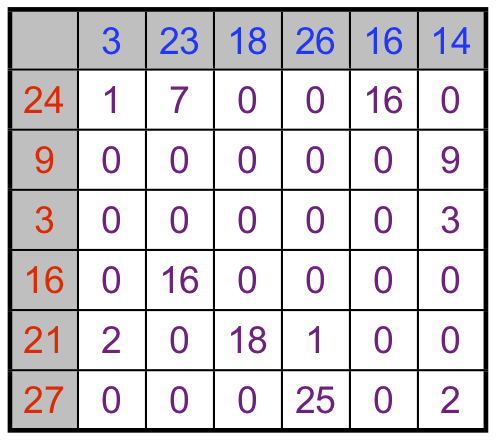
\includegraphics[width=.22\linewidth]{transport/kantorovitch/coupling-array}&
        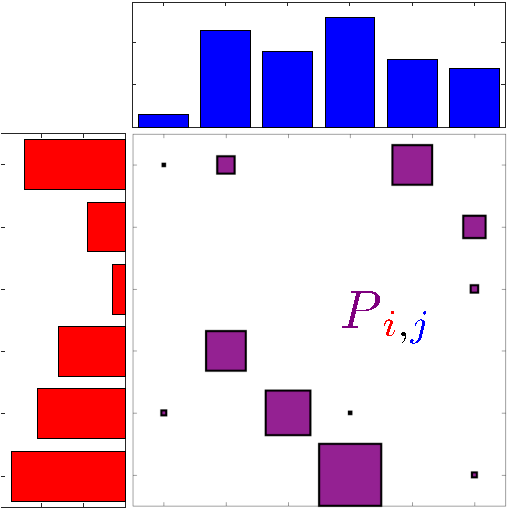
\includegraphics[width=.22\linewidth]{transport/kantorovitch/coupling-squares}&
        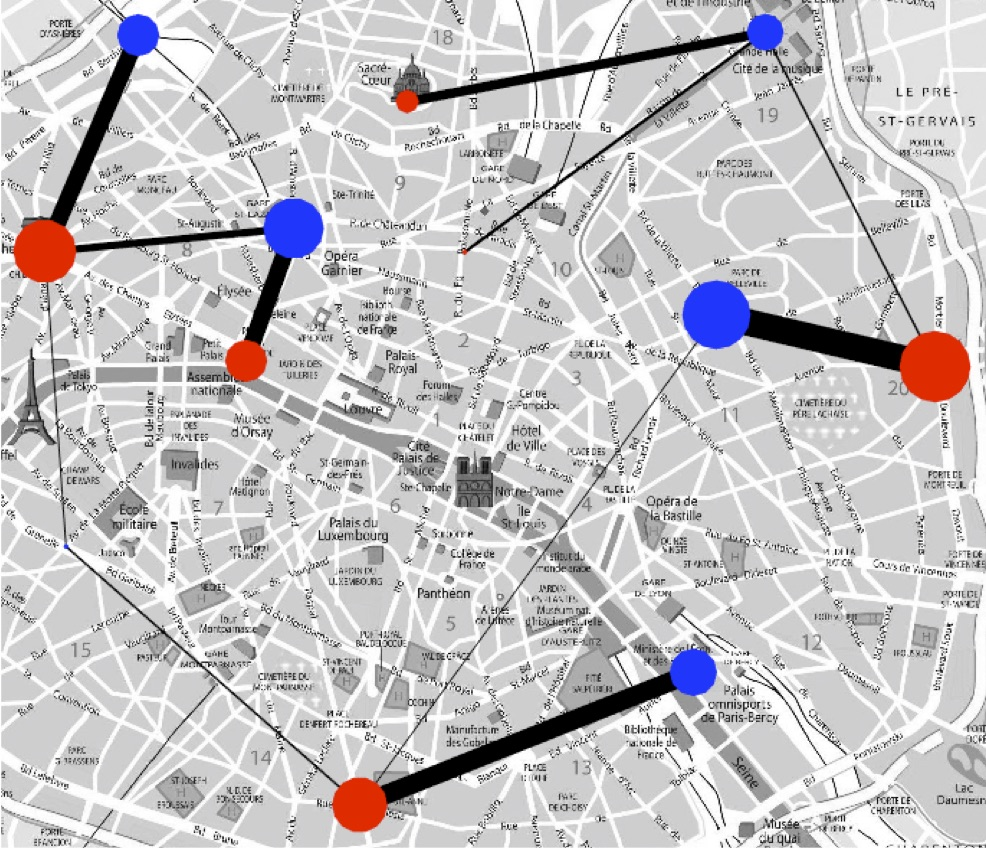
\includegraphics[width=.22\linewidth]{transport/kantorovitch/coupling-map}&
        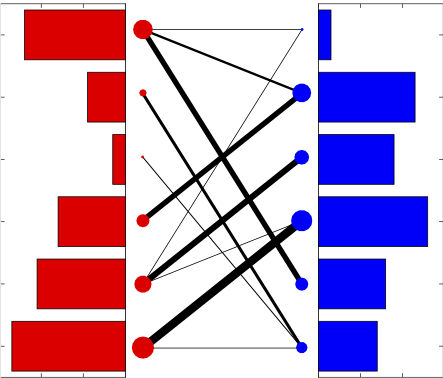
\includegraphics[width=.22\linewidth]{transport/kantorovitch/coupling-bipartite} \\
        (a) matrice & (b) histogrammes & (c) segments & (d) graphe biparti
    \end{tabular}
    \caption{\label{fig:coupling-visu} Différentes façons de représenter une matrice de couplage $P \in \Bb(\aC,\bC)$:
    	(a) un tableau de nombres dont les lignes et colonnes ont des sommes prescrites ; 
		(b) un histogramme bidimensionnel dont la taille de carré est propositionnelle à $P_{\iC,\jC}$ ; 
		(c) un ensemble de segments dont la largeur est proportionnelle est  $P_{\iC,\jC}$. 
		(d) un graphe biparti, c'est-à-dire avec deux ensembles de sommets tels que les arrêtes soient seulement entre ces deux ensembles.   } 
\end{figure}


Le problème de Kantorovitch qui généralise~\eqref{eq:kantoassign} s'écrit alors
\eql{\label{eq-kanto-gen}
    \umin{P \in \Bb(\aC,\bC)} 
        \sum_{\iC=1}^n \sum_{\jC=1}^m P_{\iC,\jC} C_{\iC,\jC}
}
ce qui signifie que l'on doit payer un coût  $C_{\iC,\jC}$ à chaque fois que l'on transfert une unité de masse entre $\iC$ et $\jC$. Tout comme le problème original~\eqref{eq:kantoassign}, on peut le résoudre de façon efficace avec l'algorithme du simplexe.  La figure~\ref{fig:coupling-visu} montre un exemple de couplage optimal. 



%%%%%%%%%%%%%%%%%%%%%%%%%%%%%%%%%%%%%%%%%%%%%%
\section{Les applications}

Bien que les motivations initiales de Monge et Kantorovitch étaient respectivement militaires et économiques, le transport optimal a trouvé d'innombrables applications, à la fois théoriques mais aussi plus concrètes. Sur le plan mathématique, on peut considérer des distributions \guill{continues} de masses, en quelque sorte la limite quand le nombre de point $n$ tend vers l'infini. Ceci permet de définir le problème de transport entre des mesures de probabilités quelconques. Ce point de vue théorique est extrêmement fructueux, et c'est le mathématicien français Yann Brenier qui a le premier montré l'équivalence dans le cadre continu des formulations de Monge et de Kantorotich~\cite{Brenier91}. Ces travaux pionniers ont montré la connexion entre le problème de transport et les équations aux dérivées partielles, et ont débouché, entre autres, sur les médailles Fields de Cédric Villani (2010) et Alessio Figalli (2018). 

\begin{figure}\centering
\begin{tabular}{@{}c@{\hspace{1mm}}c@{\hspace{1mm}}c@{}}
    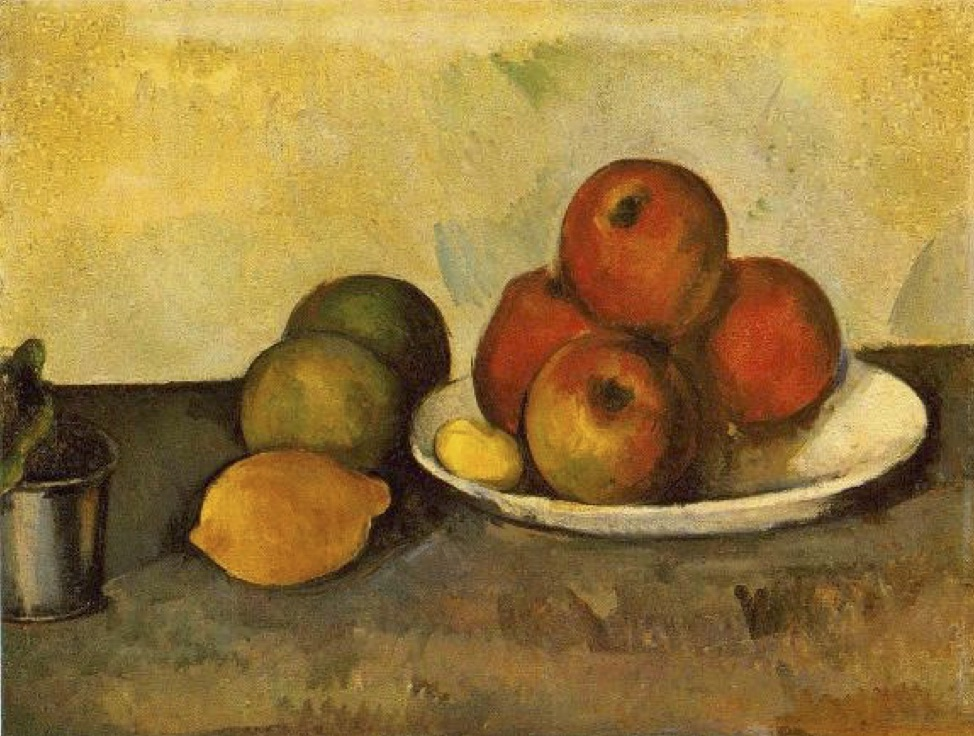
\includegraphics[width=.24\linewidth]{transport/applis/painting-2} &
    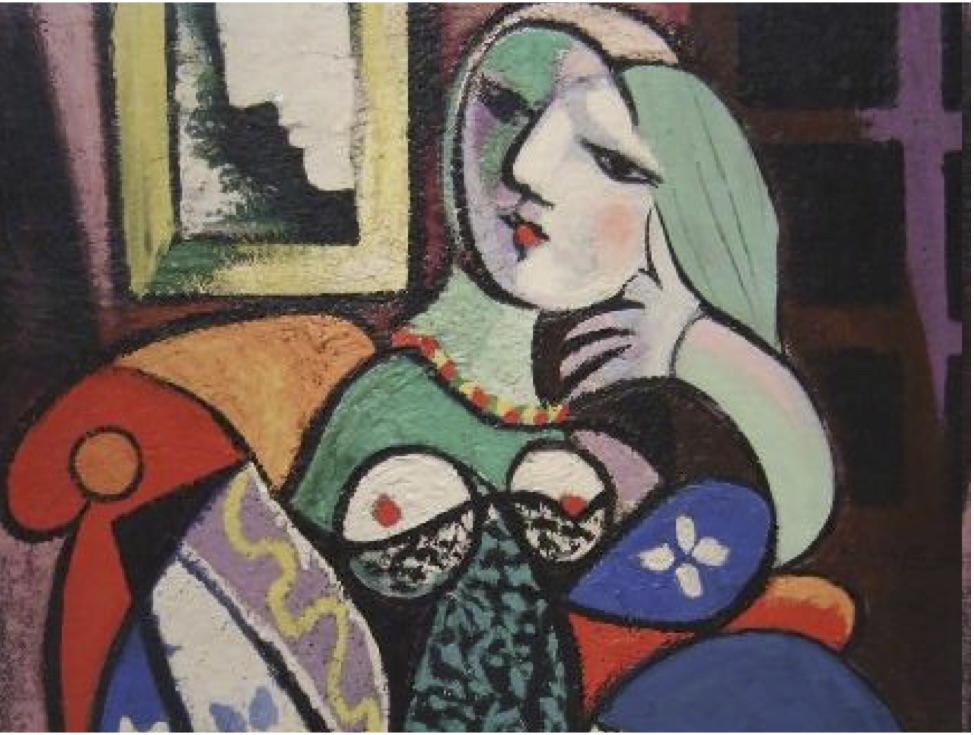
\includegraphics[width=.24\linewidth]{transport/applis/painting-1} &
    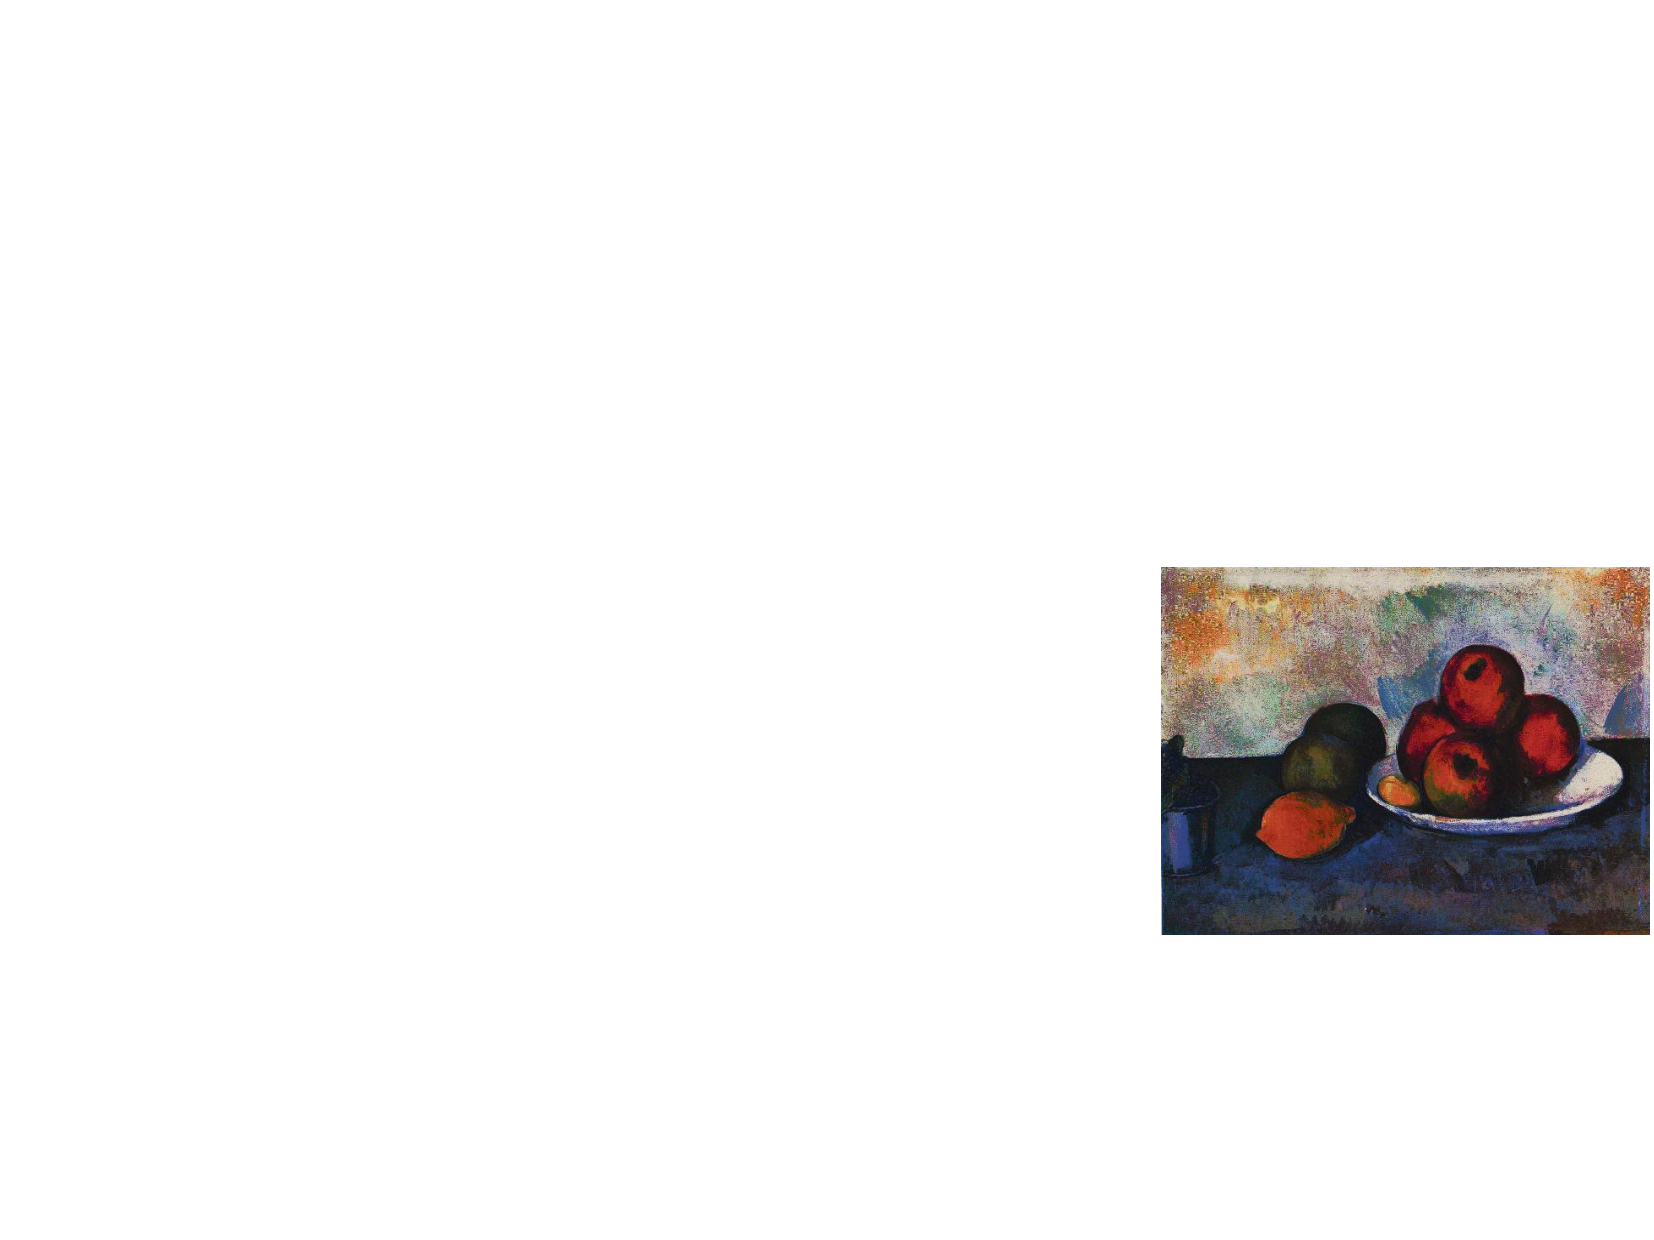
\includegraphics[width=.24\linewidth]{transport/applis/painting-2-equalized} \\
    Image $(\Red{x_i})_{\iC=1}^n$ & Image $(\Blu{y_j})_{\jC=1}^n$ & Image  $(y_{\si(\iC)})_{\iC=1}^n$ \\
    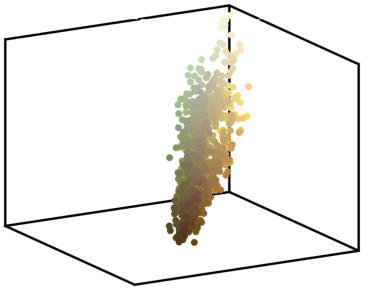
\includegraphics[width=.24\linewidth]{transport/applis/painting-2-histo}&
    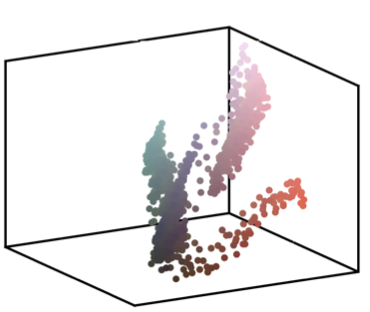
\includegraphics[width=.24\linewidth]{transport/applis/painting-1-histo}&
    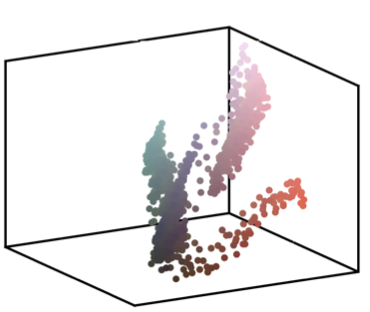
\includegraphics[width=.24\linewidth]{transport/applis/painting-1-histo}
\end{tabular}
\caption{\label{fig:image-eq} Exemple de transfert de palettes de couleurs à l'aide du transport optimal. 
	Haut: les pixels sont sur la grille d'affichage pour former une image couleur. 	
	Bas: les pixels sont placés à leurs positions dans $\RR^3$ pour former un nuage de points. }
\end{figure}

Le transport optimal est depuis peu au c\oe{}ur de problématiques plus appliquées en sciences des données, en particulier pour résoudre des problèmes en traitement d'image et en apprentissage machine. 
%
La première idée, la plus immédiate, est d'utiliser la bijection $\si$ afin de transformer des données, par exemple des images. Dans ce cas, on considère les pixels $(\Red{x_i})_{\iC=1}^n$ et $(\Blu{y_j})_{\jC=1}^n$ de deux images couleur. Chaque pixel $\Red{x_i}, \Blu{y_j} \in \RR^3$ est un vecteur de dimension 3, qui représente les intensités de chacune des trois couleurs élémentaires, rouge, vert et bleu. Afin de changer les couleurs de la première image, et lui imposer la palette de la deuxième image, on calcule le transport $\si$ pour la matrice de coût $C_{\iC} = \norm{\Red{x_i} - \Blu{y_j}}^2$ (c'est-à-dire le carré de la norme euclidienne dans $\RR^3$), c'est-à-dire le carré de la distance euclidienne entre les pixels. L'image avec les couleurs modifiées est $(y_{\si(\iC)})_{\iC=1}^n$, c'est à dire que l'on remplace dans la première image le pixel $\Red{x_i}$ par le pixel $y_{\si(\iC)}$. Cette image ressemble à la première, mais a la palette de couleurs de la deuxième image.
%
La figure~\ref{fig:image-eq} illustre ce procédé pour imposer la palette de couleurs de Picasso à un tableau de Cézanne. 

On peut également utiliser le transport optimal pour des problèmes plus difficiles, en n'utilisant que de façon indirecte la bijection $\si$ ou bien la matrice de couplage optimal $P \in \Bb(\aC,\bC)$. L'idée centrale est que la quantité associée à un couplage optimal $P$ solution de~\eqref{eq-kanto-gen}
\eq{
	W(\aC,\bC) \eqdef \sum_{i,j} P_{\iC,\jC} C_{\iC,\jC}
}
définit en quelque sorte l'effort nécessaire pour déplacer la masse de la distribution $\aC$ vers la distribution $\bC$. Elle permet donc de quantifier combien ces deux distributions sont \guill{proches}. Par exemple, si $C_{\iC} = \norm{\Red{x_i} - \Blu{y_j}}^2$ est le carré de la distance euclidienne entre des points, alors la quantité $W(\aC,\bC)^{1/2}$ est une distance entre les distributions, en particulier elle vérifie $W(\aC,\bC)=0$ si et seulement si $\aC=\bC$, et elle vérifie l'inégalité triangulaire. Ces propriétés sont très importantes pour permettre d'appliquer le transport à des problèmes pratiques.


\begin{figure}\centering
        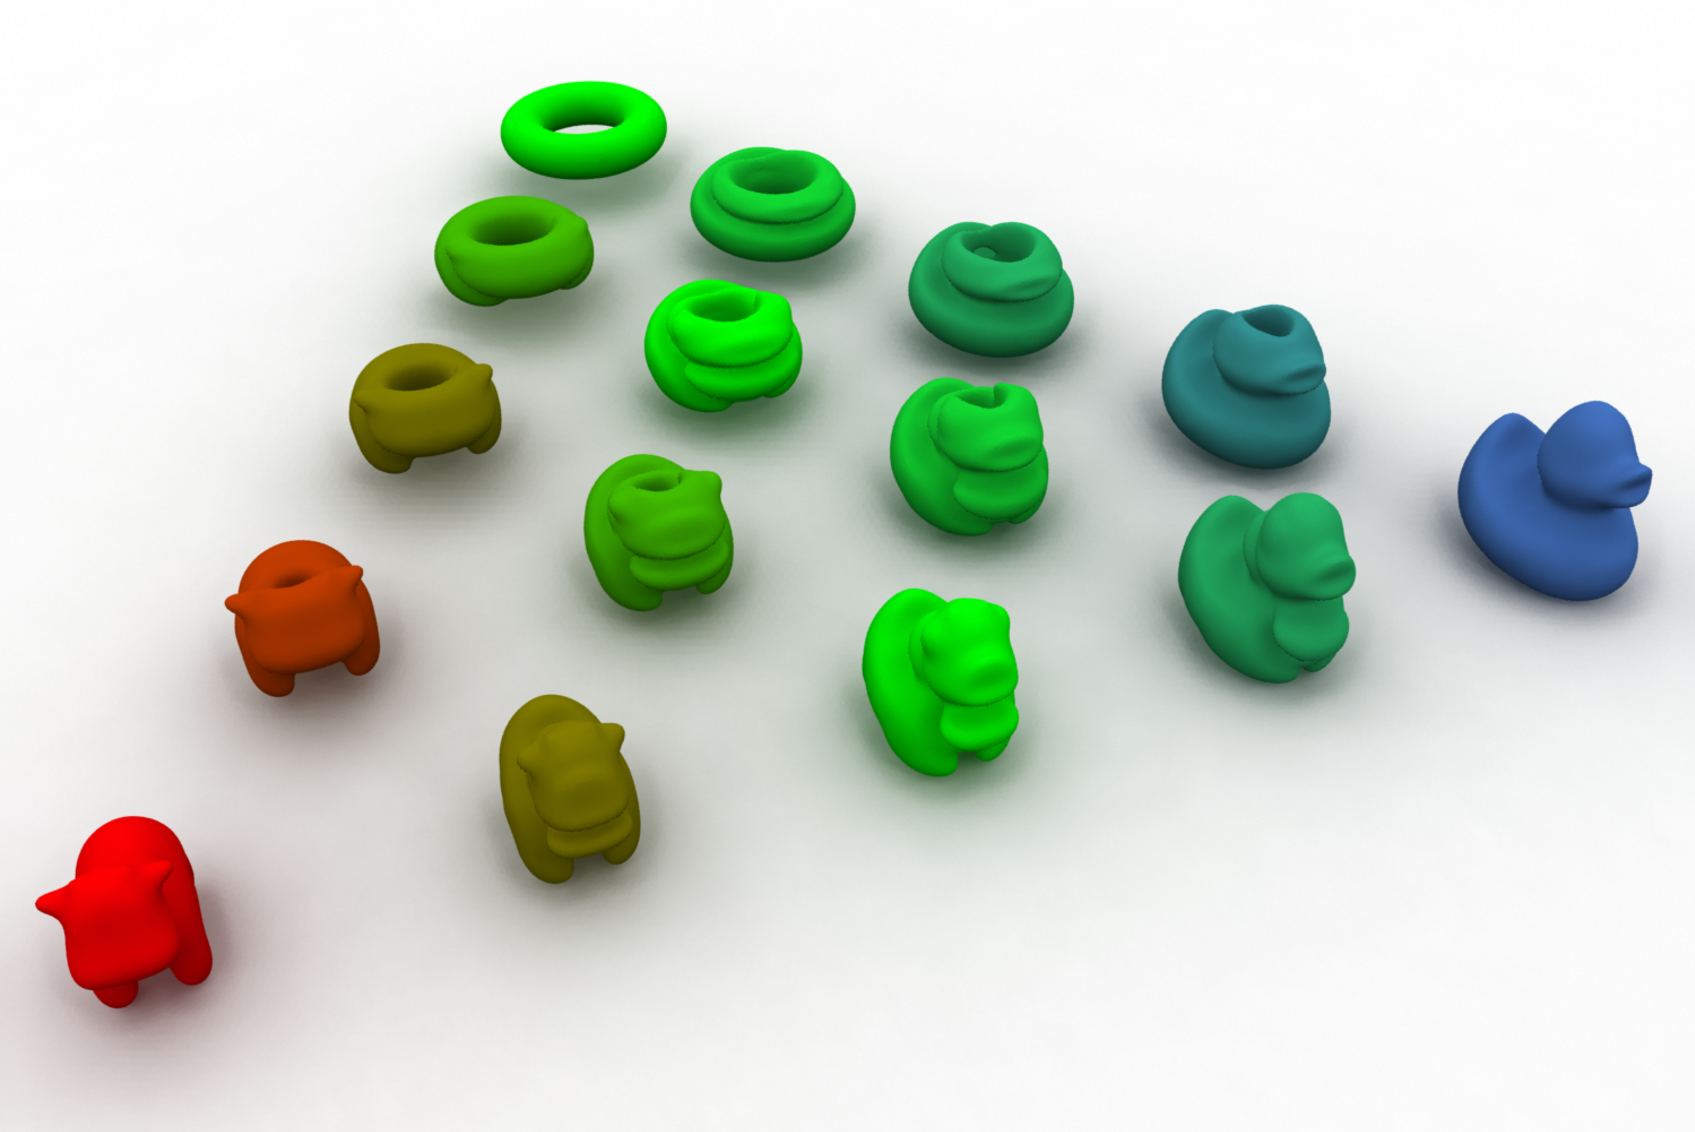
\includegraphics[width=.6\linewidth]{transport/applis/shapes-3d}
    \caption{\label{fig:barycenters} Exemple d'interpolation barycentrique entre des formes 3D, obtenu en minimisant~\eqref{eq-bary}.  }
\end{figure}

Un exemple typique d'application de cette quantité $W$ consiste à calculer des barycentres entre des distributions~\cite{agueh2011barycenters}. La figure~\ref{fig:barycenters} montre un exemple où l'on considère trois distributions $a,b,c$ (montrées aux trois sommets du triangles) qui sont des distributions uniformes de masse à l'intérieur de formes 3D (c'est-à-dire que la masse $a_i$ associée au $i^{\text{e}}$ point est 0 à l'extérieur de la première forme et prend une valeur constante à l'intérieur). 
%
On calcule un barycentre pondéré de ces trois distributions en imitant le fait que dans un espace Euclidien, le barycentre pondéré $r$ de trois points $x,y,z$ minimise la somme des distances au carré
\eq{
    \umin{r} \al \norm{x-r}^2 + \be \norm{y-r}^2 +  \ga \norm{z-r}^2,
}
où les poids $(\al,\be,\ga)$ sont les pondérations du barycentre, qui sont des réals positifs et tels que $\al+\be+\ga=1$.
%
Le barycentre pondéré $d$  de $(a,b,c)$ minimise ainsi la somme pondérée de distances de transport optimal
\eql{\label{eq-bary}
	\umin{d} \al W(a,d) + \be W(b,d) + \ga W(c,d).
}
En modifiant les poids $(\al,\be,\ga)$, on modifie la forme obtenue en se déplaçant à l'intérieur d'un triangle de transport optimal. 
%
On peut utiliser cette distance $W$ pour bien d'autres applications où l'on doit comparer des distributions de probabilité. C'est le cas en apprentissage machine, par exemple pour comparer des textes à l'aide des distributions des mots qui les composent. La figure~\ref{fig:bagwords} illustre les histogrammes d'apparition des mots pour deux textes, où la taille des lettres du mot $\iC$ est proportionnelle à la masse $\aC_\iC$. Une question difficile dans ce cas est de savoir quelle matrice de coût $C_{\iC,\jC}$ utiliser entre deux mots $(\iC,\jC)$. Il s'agit d'un travail de linguistique (caractériser la proximité sémantique entre des mots du langages), que l'on peut chercher à résoudre en même temps que le transport optimal~\cite{huang2016supervised}. 

\begin{figure}\centering
    
\includegraphics[width=.35\linewidth]{transport/applis/bag-word-1}
    \qquad
    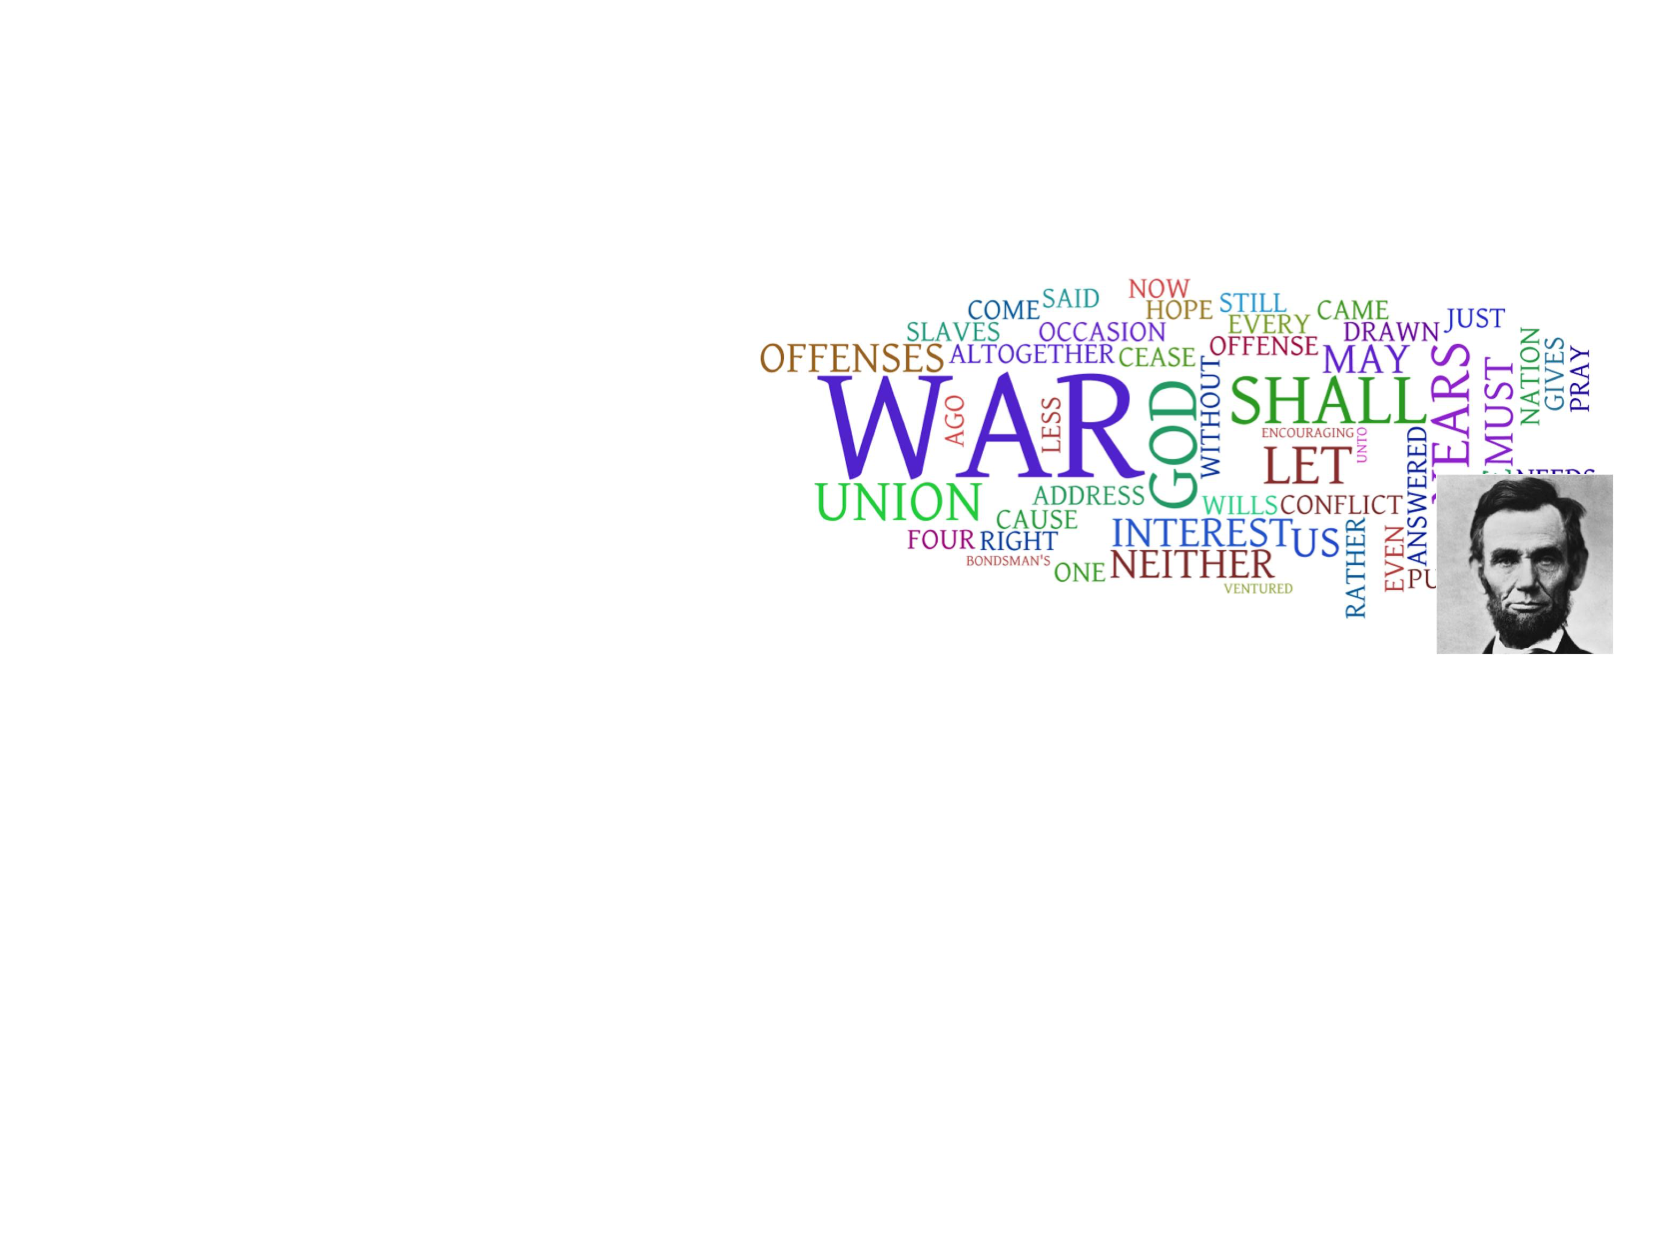
\includegraphics[width=.35\linewidth]{transport/applis/bag-word-2}
\caption{\label{fig:bagwords} Exemples d'histogrammes de distributions des mots dans deux textes différents (seuls les mots les plus fréquents sont montrés).  }
\end{figure}


%%%%%%%%%%%%%%%%%%%%%%%%%%%%%%%%%%%%%%%%%%%%%%
\section*{Conclusions}

Le transport optimal a connu de nombreuses révolutions. Sous l'impulsion de mathématiciens tels que Monge, Kantorovitch, Dantzig et Brenier, il est progressivement devenu un outil théorique et numérique fondamental. 
%
Il est maintenant au c\oe{}ur de questions importantes en science des données pour modéliser, résoudre numériquement et analyser théoriquement les problèmes de l'apprentissage machine. Les opportunités pour développer de nouvelles théories et des algorithmes performants sont immenses. 
%
Pour plus d'informations sur les aspects théoriques du transport optimal, on pourra consulter les livres~\cite{Villani03,SantambrogioBook}. Les aspects numériques et applicatifs sont couverts dans le livre~\cite{PeyreCuturi}.


%%%%%%%%%%%%%%%%%%%%%%%%%%%%%%%%%%%%%%%%%%%%%%
\section*{Remerciements}

Je tiens à remercier Vincent Beck, Gwenn Guichaoua et Marie-Noëlle Peyré pour leurs relectures attentives. 


